% Copyright (c) 2019 ETH Zurich, Integrated System Laboratory, Renzo Andri
%%%%%%%%%%%%%%%%%%%%%%%%%%%%%%%%%%%%%%%%%%%%%%%%%%%%%%%%%%%%%%%%%%%%%%%
%%%%%%%%%%%%%%%%%%%%%%%%%%%%%%%%%%%%%%%%%%%%%%%%%%%%%%%%%%%%%%%%%%%%%%%
%%%%%                                                                 %
%%%%%     <file_name>.tex                                             %
%%%%%                                                                 %
%%%%% Author:      <author>                                           %
%%%%% Created:     <date>                                             %
%%%%% Description: <description>                                      %
%%%%%                                                                 %
%%%%%%%%%%%%%%%%%%%%%%%%%%%%%%%%%%%%%%%%%%%%%%%%%%%%%%%%%%%%%%%%%%%%%%%
%%%%%%%%%%%%%%%%%%%%%%%%%%%%%%%%%%%%%%%%%%%%%%%%%%%%%%%%%%%%%%%%%%%%%%%

\chapter{Introduction}

\glsfirst{rrm} is getting more and more complex with new demands and developments like the fifth generation of mobile broadband system. Resource allocation has real-time constraints and is affected by several challenges. As machine learning has been evolved dramatically in recent years, more and more ML approaches are applied in \gls{rrm}. But these new algorithm impose new challenges on real-time embedded systems, as they are compute intense and come with high memory requirements, but also provide a lot of potential of optimization due to their regular patterns. In this project, we will research extensions for sequential machine learning models for RISC-V cores in the \gls{rrm} field and will be discussed in the following sections.

\section{Machine Learning and Sequential Models}

Even though Machine Learning has a long history, it has shown his real big break-trhough in the last few decades driven by the availability of high compute capabilities and accessibility to large datasets which made complex models more than ever trainable. 
% In general these models can be distinguished by the learning method (supervised, unsupervised, reinforced), by the sequential or non-sequential property and by the spatial dimensionality (1D feature map, 2D images, 3D images like in \glspl{ct}, etc.).

\subsection{Sequential Models}

In most common machine learning application, the data distribution is assumed to be \gls{iid} which allows to generate the likelihood function while looking at every sample point independently \cite{Bishop:2006:PRM:1162264}. But for many applications this property does not hold any more, as the data depends on time and on previous samples. E.g. in speech recognition \gls{phoneme} distributions are not \gls{iid}, but depend on the previous \glspl{phoneme}.

The most common classic sequential model is the Markov model \cite{markov1910research} where the probability distribution of a sample $\mathbf{x_N}$ can be written as a (first-order)\footnote{In a $N$-order markov chain where every sample's probability distribution depends directly on $N$ previous samples.} markov chain

\begin{align*} p(\mathbf{x_1}, ..., \mathbf{x_N}) &= p(\mathbf{x_N})\cdot \prod^N_{n=2} p(\mathbf{x_n}|\mathbf{x_{n-1}}), \\
p(\mathbf{x}_n|\mathbf{x}_1, ..., \mathbf{x}_{n-1})&=p(\mathbf{x}_n|\mathbf{x}_{n-1})
\end{align*}
whereas every sample $x_N$ directly depends on its predecessor  $x_{N-1}$  \cite{Bishop:2006:PRM:1162264}. An extension to this model are \glspl{hmm} with discrete states and where the state can not be observed directly, but the output. These models have been used in speech recognition, natural language modelling, on-line handwriting recognition and analysis of biological sequences (e.g. proteins, and DNA) \cite{Bishop:2006:PRM:1162264}.

\subsection{Feedforward Neural Networks}
Artificial Neural Networks are brain-inspired models, which traditionally consist of a set of input neurons $\mathbf{x}\in \mathbb{R}^k $, hidden units $\mathbf{h}\in \mathbb{R}^l$ and output neurons $\mathbf{y}\in \mathbb{R}^m$ and the neurons are connected by synopses (or vertices), each of which is assigned a weight value $W_h(k,l)$  and $W_y(l,m)$ which is the contribution of the input neurons to the output neurons. The activation or transfer function $\sigma_h$ and $\sigma_y$  (e.g. Rectified Linear Unit ReLU\footnote{The ReLU activation function can be expressed as follows: $\sigma_{ReLU}(x)=max(0, x)$}) is used to determine the state of $\mathbf{h}$ and  $\mathbf{y}$ based on its input neurons and introduces non-linearity in the network which enables to learn non-simple tasks. The most basic neural network block is the \gls{mlp} which has at least three layers: an input and output neuron layer and a (fully-connected\footnote{All input neurons contribute to all output neurons}) hidden layer and can then be represented as the follows:
\begin{align*} 
\mathbf{h}&= \sigma_h(W_h\mb{x}+\mb{b}_h)\\
\mathbf{y}&= \sigma_y(W_y\mb{h}+\mb{b}_y)
\end{align*}
Typically several hidden layers are stacked together. Another special case are \glspl{cnn}, where the spatial dependency (translation invariance and correlation of neighboring pixels) of the input and hidden units is exploited and a convolution kernel is learned per input and output neural layers instead of a weight for every neuron.
Feedforward Neural Network have no dependency of previous samples and therefore do not have any cyclic paths in the network which makes them (comparably) simple to train, but are not so common to learn data with sequential dependency.

\subsection{Recurrent Neural Networks RNN}
To also take the sequential property of data (e.g. audio samples) into account, recurrent neural networks introduce recurrent vertices into the network, as illustrated in Fig.~\ref{fig:rnn} where as $U_{h}\in \mathbb{R}^{m\times m}$ are the recurrent weights of a single-layer RNN.

The network can then be written as:

\begin{align*} 
\mb{h}_t &= \sigma_h(W_{h} \mb{x}_t + U_{h} \mb{h}_{t-1} + \mb{b}_h) \\
\mb{y}_t &= \sigma_y(W_{y} \mb{h}_t + \mb{b}_y)
\end{align*}

\begin{figure}[ht]
    \centering
    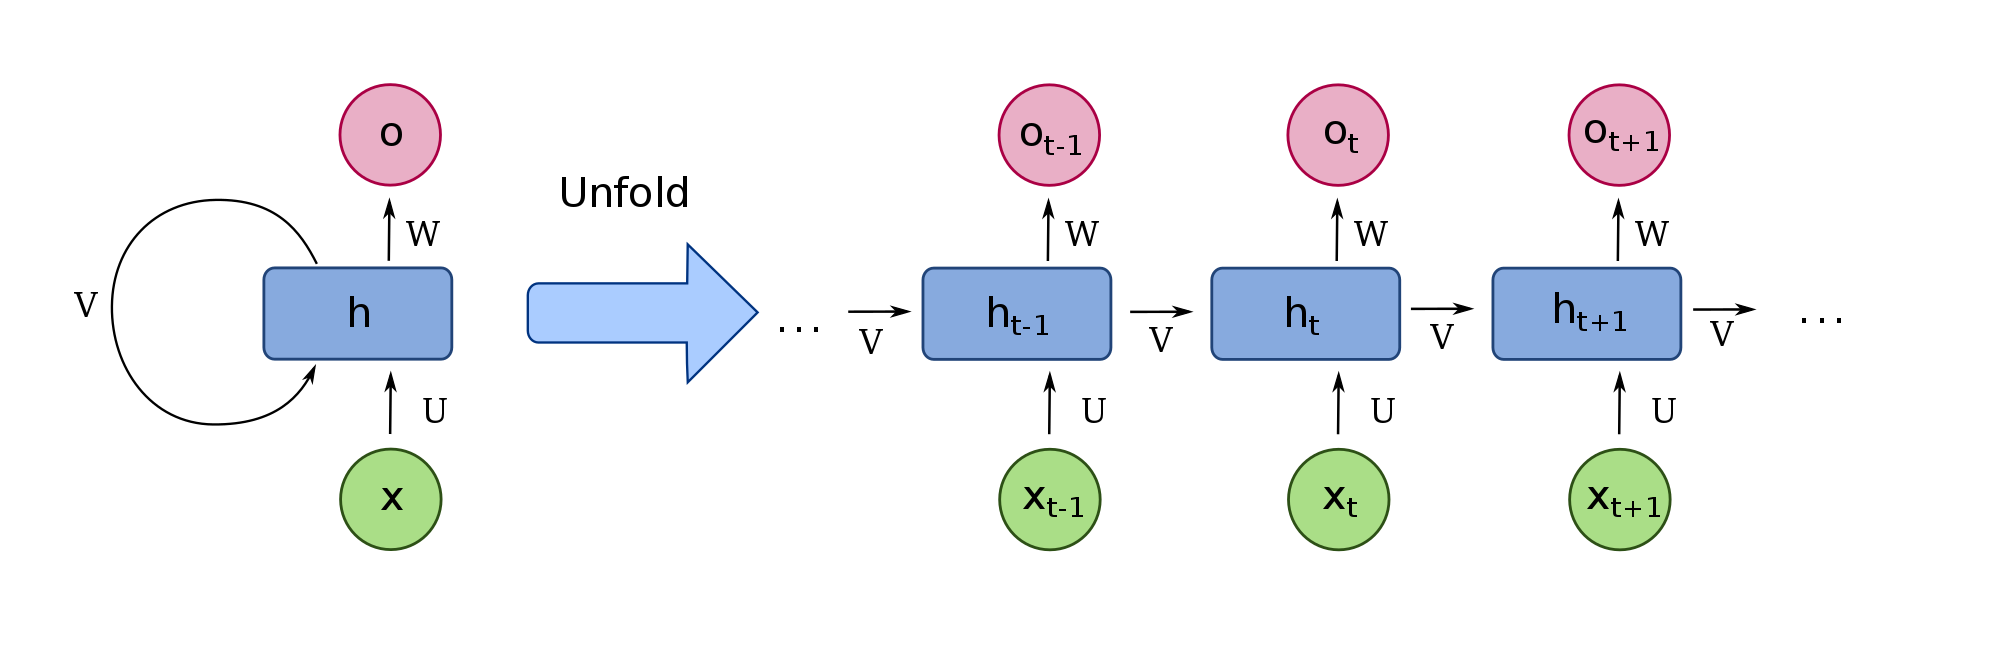
\includegraphics[width=\textwidth]{figures/rnn.png}
    \ifdefined\SHOWNOTES
    \caption{RNN cell unfolded in time \cite{wikimediaRnn} }
    \else
     \caption{RNN cell unfolded in time \cite{wikimediaRnn}}
     \fi
    \label{fig:rnn}
\end{figure}

\gls{rnn} can support variable length in sequential model, but suffer from vanishing gradient problem during training making training slow and long-term dependencies hard to train.

RNN have been trained on a large set of applications, e.g. to create automatic image caption \cite{karpathy2015deep}, text generation like poems, wikipedia article, linux kernels and language translation \cite{sutskever2011generating}.  

\subsection{Long Short-Term Memory}
Hochreiter and Schmidhuber introduced \glspl{lstm} where an additional internal memory cell $\mathbf{c}_t$ and a forget gate $\mathbf{f}_t$ is inserted to a standard RNN. LSTM has been shown to be much less prune to the vanishing gradient problem and can therefore learn much longer time-dependencies\cite{hochreiter1997long}. The following formula and Fig.~\ref{fig:lstm} show the structure of a typical LSTM cell unfolded in time.

\begin{align*}
f_t &= \sigma_g(W_{f} x_t + U_{f} h_{t-1} + b_f) \\
i_t &= \sigma_g(W_{i} x_t + U_{i} h_{t-1} + b_i) \\
o_t &= \sigma_g(W_{o} x_t + U_{o} h_{t-1} + b_o) \\
g_t &= \sigma_c(W_{c} x_t + U_{c} h_{t-1} + b_c) \\
c_t &= f_t \circ c_{t-1} + i_t \circ g_t  \\
h_t &= o_t \circ \sigma_h(c_t)
\end{align*}

with the following activation functions:\\
$\sigma_g$: sigmoid function\footnote{sigmoid function: $\sigma_g(x) = \operatorname{sig}(x) = \frac{1}{1 + e^{-x}}$}\\
$\sigma_c$: hyperbolic tangent\\
$\sigma_h$: hyperbolic tangent or identity.\\

\ifdefined\SHOWNOTES
\textbf{maybe some examples}\\
* Alex Graves, Geoffrey Hinton, Speech Recongition with deep recurrent neural networks [18]
    * e.g. PreTrans-3L-250H $\rightarrow$ **3 layers** with **250 LSTM** hidden (bi-directional LSTM) cells with **4.3 Mparam**
    * Phoneme recognition on [TIMIT corpus](https://www.sciencedirect.com/science/article/pii/0167639390900107)
    * RNN lib by Graves (https://sourceforge.net/p/rnnl/wiki/Home/)
* [Bahdanau, Dzmitry, Kyunghyun Cho, and Yoshua Bengio. « Neural machine translation by jointly learning to align and translate. » arXiv preprint arXiv:1409.0473 (2014).](https://arxiv.org/pdf/1409.0473.pdf)
    * GRU only??
    * Encoder and Decoder LSTM networks $\rightarrow$ translate from english to french to another based on [Cho et al.](Cho et al. 2014a), [Sutskever et al.](Sutskever et al. 2014 ) 
    * separate network for attention weights
    * no repo available, dataset available \url{(http://www-lium.univ-lemans.fr/~schwenk/cslm_joint_paper/)}
    * **1000 cells per layer**, word embedding with 620 features
* Graves, Alex, et al. "A novel connectionist system for unconstrained handwriting recognition." IEEE transactions on pattern analysis and machine intelligence 31.5 (2009): 855-868.
    * Bidirectional LSTM for handwriting recognition
    * **25 input neurons, 2 layers (backwards and forwards)** with **100 LSTM** blocks each
* Wu, Yonghui, et al. "Google's neural machine translation system: Bridging the gap between human and machine translation." arXiv preprint arXiv:1609.08144 (2016).
    * 1024 LSTM nodes per layer
    * encoder, decoder and attention network
* Challita, Ursula, Proactive Resource Managemtn in LTE\_U Systems: A Deep Learning Perspective
    * Traffic encoder  (LSTM)followder by MLP followed by action decoder (LSTM)

\fi

\begin{figure}[ht]
    \centering
    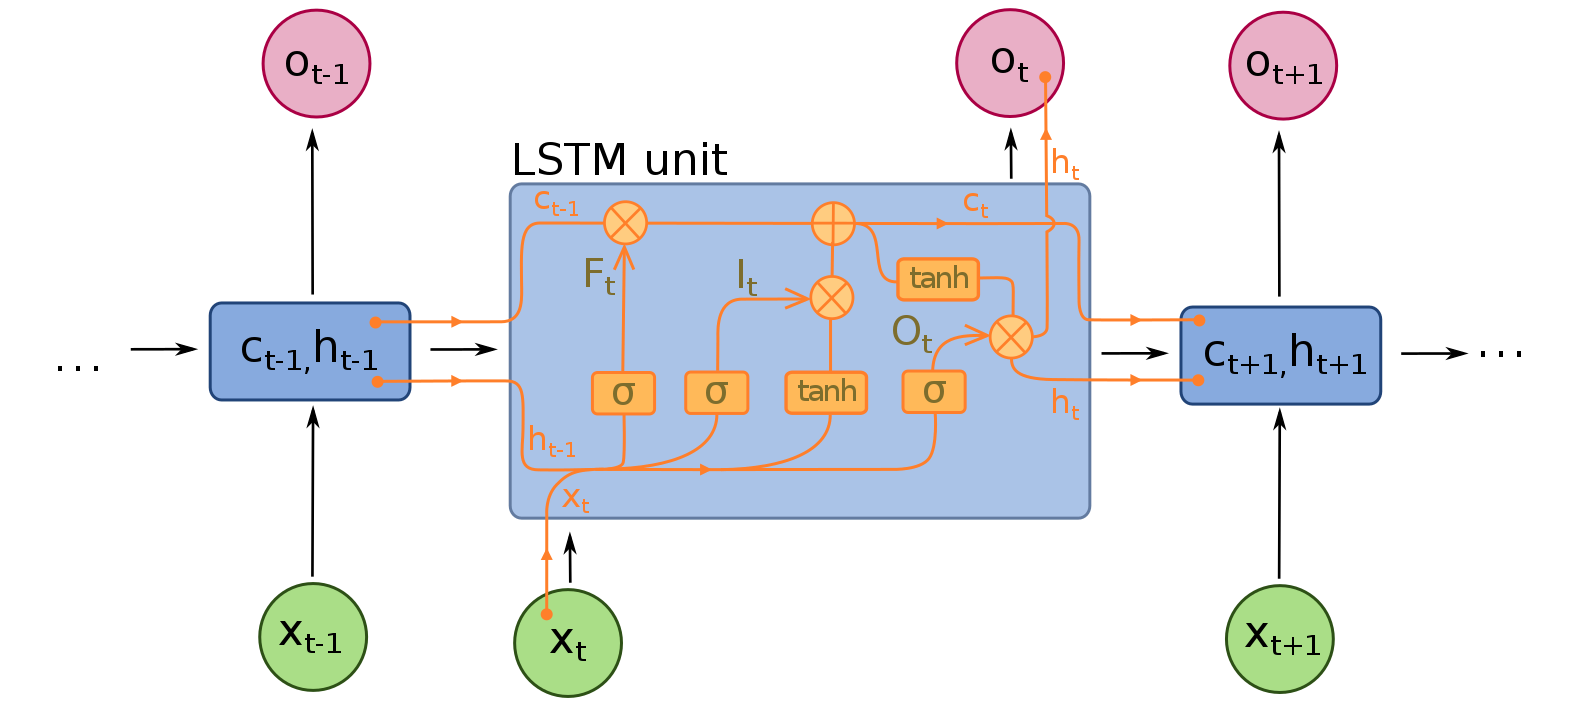
\includegraphics[width=\textwidth]{figures/lstm.png}
    \caption{LSTM cell unfolded in time \cite{wikimediaLstm}}
    \label{fig:lstm}
\end{figure}

\subsection{Gated Recurrent Units}
\gls{gru} are a simplified version of LSTMs which have no separate output gate and therefore have less computations and parameters. Similar results have been shown than with LSTMs \cite{bahdanau2014neural}, although no extensive study has been conducted yet. The GRU is illustrated in Fig.~\ref{fig:gru} and formalulated in the following equations:
\begin{align*}
z_t &= \sigma_g(W_{z} x_t + U_{z} h_{t-1} + b_z) \\
r_t &= \sigma_g(W_{r} x_t + U_{r} h_{t-1} + b_r) \\
h_t &=  (1 - z_t) \circ h_{t-1} + z_t \circ \sigma_h(W_{h} x_t + U_{h} (r_t \circ h_{t-1}) + b_h)\\
\sigma_g(x) &= \operatorname{sig}(x), \sigma_h(x) = \operatorname{tanh}(x) 
\end{align*}

\begin{figure}[ht]
    \centering
    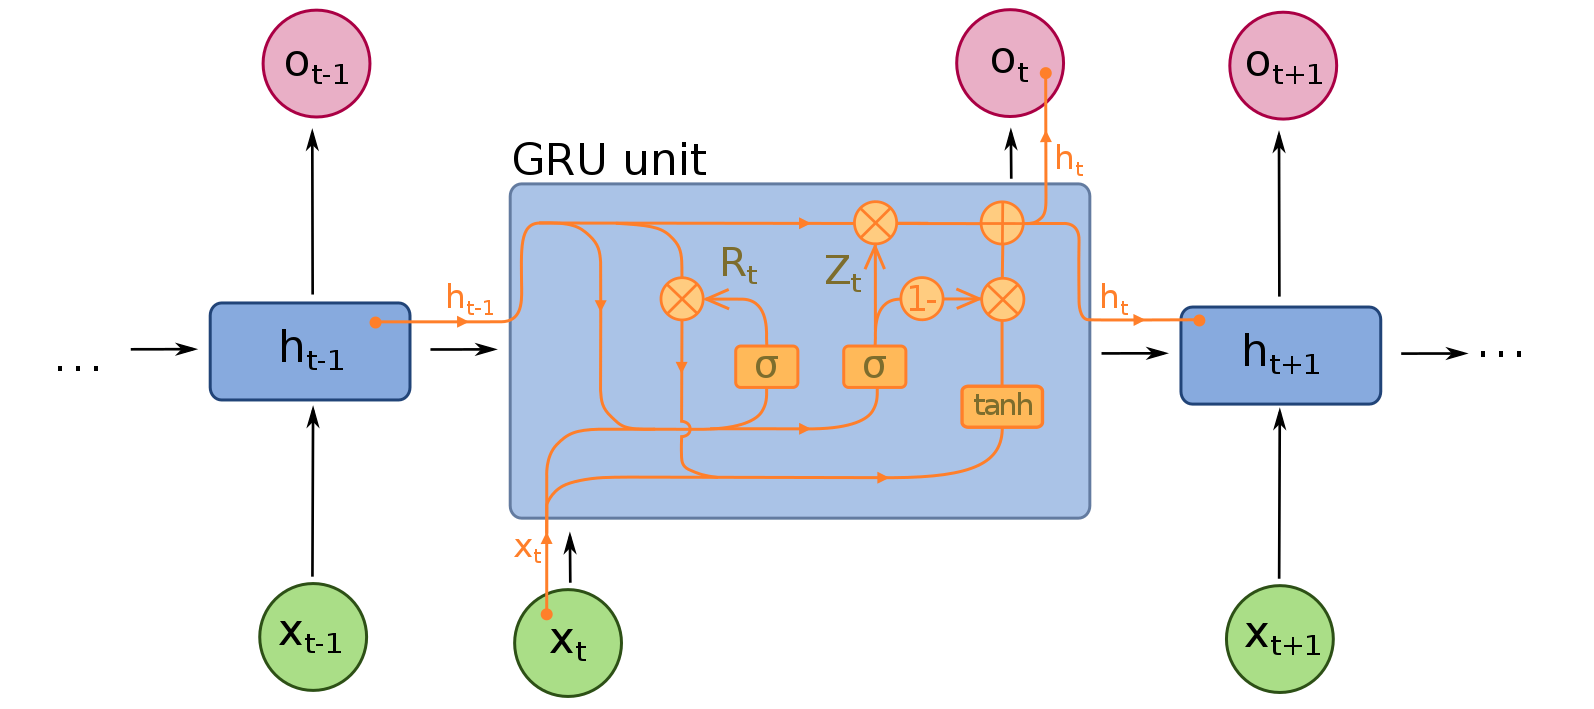
\includegraphics[width=\textwidth]{figures/gru.png}
    \caption{GRU cell unfolded in time \cite{wikimediaGru}}
    \label{fig:gru}
\end{figure}

\subsection{Dilated Causal Networks}
Recurrent paths make training much harder than in fully-feed forward networks, an alternative presented by Cheema et al. are Dilated Causal Networks, where time is encoded into the 1-d input feature space \cite{cheema2018dilated}. Additionally, the data is fed through the network in a logarithmic way, as illustrated in Fig.~\ref{fig:dilated} to support a wide range of sequential dependency in the input data. These networks have been used for training motion detection \cite{cheema2018dilated} and machine translation \cite{kalchbrenner2016neural} and on a set of common sequential model tasks \cite{bai2018empirical} with slightly better performance and with much fast convergence compared to recurrent models.

\ifdefined\SHOWNOTES
\begin{itemize}
    \item Dilated Temporal Fully-Convolutional Network for Semantic Segmentation of Motion Capture Data, June 2018 \cite{cheema2018dilated}.
    \begin{itemize}
        \item motion detection with 5 convolution layers in dilated order
        \item 3x3 conv in first layer, 1d convs in further layers (temporal and acausal)
        \item 663 k parameters
    \end{itemize}
    \item Kalchbrenner et al. (Deepmind), Neural Machine Translation in Linear Time (ByteNet), March 2017
Machine Translation \cite{kalchbrenner2016neural}
    \begin{itemize}
        \item 30 (non-standard) residual blocks (split into 6 sets of 5 blocks, each block with different dilation rates), 512 hidden units
    \end{itemize}
    \item An empirical evaluation of generic convolutional and recurrent networks for sequence modeling
\cite{bai2018empirical}

\end{itemize}
\fi


\begin{figure}[ht]
    \centering
    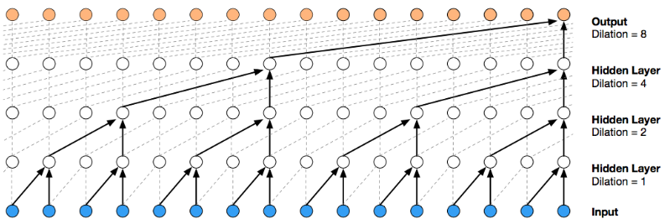
\includegraphics[width=0.7\textwidth]{figures/dilated.png}
    \caption{Dilated Causal Networks \cite{cheema2018dilated}}
    \label{fig:dilated}
\end{figure}

\subsection{Spectrogam-based (Convolutional) Neural Networks}
Sequential data can also be represented in a spectrogram, where as a sliding window of sequential samples are mapped to the frequency domain using FFT. The resulting time-to-frequency image is than fed to a  conventional convolutional network and has been used for speech recognition \cite{abdel2012applying}.
\ifdefined\SHOWNOTES
\subsection{Other potential sequential models}
The following list gives a short introduction in other potential networks:

\begin{itemize}
    \item Bidirectional RNN: usually a backward network and a forward network which allows also from future samples (e.g. in machine translation predicting the first word may profit when we already know a future word). These networks are not really causal anymore and are not so suitable for reactive systems.
    \item Recurrent Convolutional Neural Netorks RCNN: RNNs but the spatial dependence between neighboring features are exploited.
    \item Multi-dimensional RNN:
    \item Unitary Recurrent Neural Networks: Unitary transfer matrices are enforced ($U^HU=I$).
    \item Gated Orthogonal Recurrent Unit: Orthogonal transfer matrices are enforced.
    \item Grid LSTM \url{https://arxiv.org/pdf/1507.01526.pdf}
    \item Differential Recurrent Neural Networks
    %\item Neural Turing Machine
\end{itemize}
\fi
\subsection{Reinforcement Learning and Q-Learning}
Q-Learning is a reinforcement learning technique. Typically, the model setup includes an agent in a environment, which can have a set of states $s\in S$ and can apply an action of a set $a\in A$. After applying action $a$, the environment returns a reward $r\in R$ back to the agent.

The action policy learned in Q-Learning is represented by the Q-function $Q: S \times A \to \mathbb{R}$ mapping state action pairs to the expected reward. The learning procedure happens iteratively by updating Q in the following way:\\

\[Q_{k+1}(s_{t},a_{t}) \leftarrow (1-\alpha) \cdot Q_{k}(s_{t},a_{t}) + \alpha \cdot  \bigg( r_{t} + \gamma \cdot \max_{a\in A}Q(s_{t+1}, a) \bigg) \]

where as $\alpha$ is the learning rate and $\gamma$ accounts for future rewards. Typically the agent applies the action which has the highest Q values for the current state (exploitation) or selects a random action (exploration) \cite{mnih2015human}. 

In traditional Q-Learning an extensive Q table is learned including all $|S|\cdot|A|$ possible entries. Recent works instead suggest to learn a (deep) neural network to represent the Q function, also known as \gls{dqn} \cite{mnih2015human}.

\textbf{Dueling DQN DDQN}\\
In dueling DQN Q function is split into the state value $V(s)$ and the advantage value $A(s,a)$, where as
$Q(s,a)=A(s,a)+V(s)$. Both values are being learned by two separate neural networks \cite{wang2015dueling}. DDQN can better account for cases, where the state is either good or bad independently from the taken action.

\ifdefined\SHOWNOTES
% Experience replay to enhance learning of DQNs...
\fi
\ifdefined\SHOWNOTES
\section{hidden notes}
   \begin{itemize}
    \item \cite{juang2005automatic} Automatic speech recognition - history 
    \begin{itemize}
        \item 
    \end{itemize}
\end{itemize}
\fi

\section{Radio Resource Management (RRM)}
Wireless communication is omnipresent nowadays and the desired data total bandwidth is driven by the increasing number of devices (e.g \gls{iot} end nodes and smartphones) and the increasing requirements of the applications (e.g. virtual reality, video-telephony). \gls{rrm} manages the allocation of radio resources (e.g. bands, transmit power, data rates, modulation, error coding schemes, ...) in a multi-cell and multi-user setting which imposes crosstalk from other radio transmitters (\gls{cci}), especially as publicly available frequency bands are limited \cite{tripathi2006radio}.

Implementing the \gls{rrm} efficiently imposes several challenges: The clients are heterogeneous (e.g. tiny sensor-nodes vs. mobile routers) and clients are moving within and between network cells. Parameter space is high-dimensional and components within the network are varying and state changes are happening stochastically. Especially, theses tasks have to be executed in the frame of milliseconds which exclude compute-intense algorithms \cite{Sun2017}. Additionally, radio cells are overlapping and observability and controllability of the entire system is limited \cite{Ghadimi2017}. 

Typically, the system has been modelled with full observability and optimizing convex problems with algorithmic\cite{Sun2017} approaches like the weighted sum-rate MSE algorithm\cite{shi2011iteratively} and fractional programming \cite{naeem2013optimal} which are calculated in an iterative way and some of them need to calculate heavy operations (e.g. matrix inversion or singular value decomposition) in every iteration.

\ifdefined\SHOWNOTES
well known optimization based algorithms: developed for power control (e.g. iterative water-filling tzpe algorithms, interference pricing, SCALE), transmit receive beamformer design (e.g. wmmse algorithm, pricing ased scheme, semidefinite relaxation, admission control (e.g. the deflation based schemes, convex approximation based schemes), user/base station clustering...from\cite{Sun2017}
\fi

As these systems would profit from a reactive learning setting, also reinforcement learning approaches have been applied. Q-Learning with a single agent \cite{galindo2010distributed,yau2009context,vu2018ultra} or multi-agent setting with distributed agents \cite{Ghadimi2017,calabrese2016learning,amiri2018machine} or centralized agents \cite{Nasir2018}. Beside of the classic Q-learning approach \cite{bennis2010q,simsek2011improved}, also deep Q-networks have been presented using feedforward neural networks \cite{Ye2017,Ghadimi2017,Yu2017,Nasir2018} or \glspl{lstm} \cite{Naparstek2017}.

\chapter{Benchmarks}
To evaluate several relevant implementations and extensions for sequential models on RISC-V cores in the \gls{rrm} field, we have selected several recent publications, which are described in Table~\ref{tab:benchmarks}. Even though the optimization objectives of these networks are different (e.g. throughput/spectral efficiency maximization, interference reduction, fair allocation), the network topology and learning procedure are similar, but differ mainly in the kind of network layers (\gls{lstm}, feedforward neural networks (\gls{mlp} and \gls{cnn}) and the learning method (supervised learning or reinforcement learning with DQN). 
Not all of the papers have published the exact setup (e.g. number of access nodes or frequency bands) and therefore also not all relevant network parameters (e.g. input and output neurons). In the following, the number of antennas is set to $K=4$ and the number of frequency bands to $N=3$ otherwise indicated in the paper.

\section{Proactive Resource Management in LTE-U Systems: A Deep Learning Perspective \cite{Challita2017}}
Challita et al. have presented a learning framework in the field of \gls{lte-u} (4G), where as \gls{sbs}\footnote{low-powered cellular radio access nodes with a range of 10\,m to 1\,km, few concurrent connections/sessions} are sharing unlicensed bands. The number of bands is rather small, therefore fair and an altruistic policy is needed and should be learned. The SBS are not collaborating directly, but try to achieve long-term fairness measured in average airtime per radio while optimizing proactively dynamic channel selection, carrier aggregation and fractional spectrum access. Challita et al. show that they reach a mixed-strategy Nash equilibrium and can gain up to 28\% over a conventional reactive approach. They use a combination of LSTMs and MLP: The state encoder tries to reconstruct the predicted action sequence and is modeled with a one-layer LSTM with 70 cells, followed by a summarizing fully-connected layer with unknown size and has been set to the same size (i.e. 70) and is followed by the action decoder modelled by a one-layer \textbf{70 cell} LSTM with $K=4$ output neurons. 


\iffalse
\begin{itemize}
    \item Challita et al. \url{https://arxiv.org/pdf/1702.07031.pdf}
    \item \gls{lte-u} (4G) \follows using the free frequencies, but need to co-exist with WiFi
    \item resource allocation problem of LTE-U with small (cell) base stations SBS\footnote{low-powered cellular radio access nodes with a range of 10m to 1km, few concurrent connections/sessions}
    \item multiple SBS performing proactively dynamic channel selection, carrier aggregation and fractional spectrum acces while guaranteeing fairness with existing WiFi networks and other LTE-U operators.
    \item SBS modelled as homo egualis\footnote{Homo Egualis are considered agents (or humans) being totally altruistic.\cite{arslan2007cognitive}} aiming to predict future actions and thus achieving long-term fairness (based on average airtime per radio)
    \item no cooperation \follows utilize past observations to build predictive models on spectrum availability and to intelligently plan channel usage over a finite time window.
    \item shown to reach a mixed-strategy Nash equilibrium
    \item 28\% gains over a conventional reactive approach
    \item encoder, decoder network with lstm \follows traffic encoder takes as an input the historical traffic loads and learns a vector representation of tinpute time series..., mlp to summarize. The action decoder tries to reconstruct the predicted action sequence. Fig.~\ref{fig:challita_mod} shows the network which was used, it is made up of three components a traffic encoder network creating, a summarizing network and an action decoder. 
    \item 1 hidden layer, more layer didn't help
    \item dataset wifi traffic load and sbs traffic load collected over "several" days. (testing on real setting)
    \item contention-based protocol \follows measure state of channel first (idle, busy)
    \item REINFORCE algorithm for gaussian policy \[challita/26\]
    \item issue not known MLP network
\end{itemize}
\begin{figure}
    \centering
    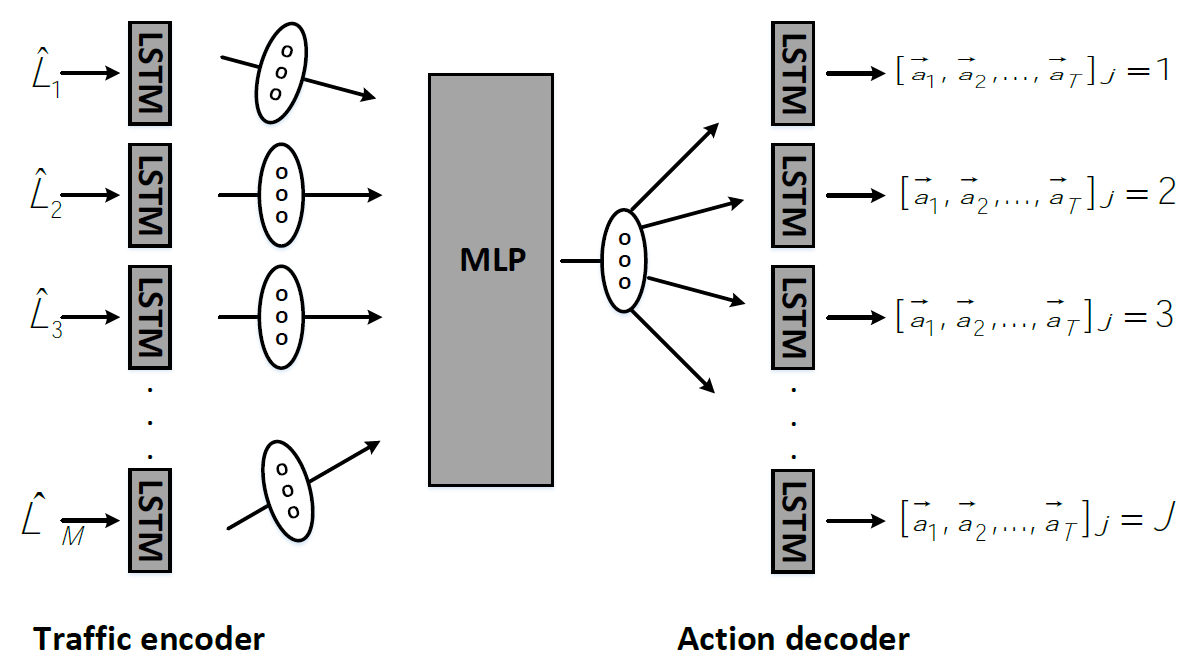
\includegraphics[width=0.8\textwidth]{figures/challita1.png}
    \caption{Learning Framework \cite{Challita2017}}
    \label{fig:challita_mod}
\end{figure}
\fi

\section{Deep Multi-User Reinforcement Learning for Distributed Dynamic Spectrum Access \cite{Naparstek2017}}
Naparstek et al. apply Deep Q-Learning to solve the \gls{dsa} utilization problem. The time is slotted into fixed-size times slots and each user selects a channel and transmits a packet with a certain attempt probability. After each slot, the user gets an acknowledgement whether the transmission was successful or not. The problem is learned with a DQN approach, where as the network consists of $(2N+2)$ input neuron where the first $(N+1)$ neurons is encoding the last channel selected and the other $(N)$ encodes the capacity of the $N$ sub-bands and 1 for the acknowledge signal. These neurons connect to a single-layer LSTM with unknown size (i.e. set to $2N+2$), and finally fed through two independent linear layers (the value layer and the advantage layer) based on the dueling DQN principle; both layers have $N+1$ output neurons each. As the exact network topology has not been published, the number of layer is set to 1. Based on double Q learning, the network is trained separately to choose the action and to estimate the Q-value associated to the according action.

\ifdefined\SHOWNOTES
\begin{itemize}
    \item Naparstek et al.
    \item maximization of utilization
    \item synchronized time slot, each user selects a channel and tramsmit a packet with a certain attempt probability, after each slot, local observation successfull or not
    \item multi-user without online coordination or inter-user communciation
    \item problem: large state space (especially for extensive q-learning) and partial observability
    \item distributed dynamic spectrum access algorithm based on deep multi-user reinforcement learning
     reinforcement learning an overview of y.li
    \item adjust transmission parameters (e.g. which channel, attempt probaility to use) \follows maximizing network utility
    \item is able to adapt to topology changes, different objectives, and different finite time-horizon (where dynamic programming is intractable)
    \item while offline, \follows training the multi-user dqn at a central unit to max. the objective on a centralized powerful unit
    \item random access control, every node has always data to send, but send with an attempt probability
    \item $K$ channels available \follows input layer with $(2K +2)$ elements, where as the first (k+1) elements used to indicate which channel has been used (just 1 channel can be selected), the other k+1 is indicating the capacity of the channel (e.g. throughput), one element for the acknowledgement signal.
    \item to learn hwo to aggregate experiences over time \follows lstm 
    \item use of dueling DQN (+ double q learning spliting the dqn to evaluate q and the selection of action to reduce selecting overestimated values \follows overoptimistic values
    \item reading suggestion: a survey of dynamic spectrum access from Yhao and sadler or multiagent-learning for aloha-like spectrum access in cognitive radio systems from h li.or deep
\end{itemize}
\fi
\section{Deep reinforcement learning for resource allocation in V2V communications\cite{Ye2017}}
Ye et al. elaborate the resource allocation problem in vehicle-to-vehicle and base station-to-vehicle communication setup (e.g. information on traffic safety). Every vehicle is an agent deciding independently to reach an optimal band and power level selection. The system is modeled in a Q-Learning setup where as the reward is determined by latency and reliability metrics, the state is based on the channel information of the corresponding link, previous interference on the link, channel information to the base station, selected sub-channel of neighbors in the previous time slot, the remaining load to transmit and the remaining time to meet latency constraint. The actions are the sub-band to select and transmission power. The Q function is then learned and modelled by a \textbf{5 layer fully-connected} neural network with 500,250,120 hidden neurons. There are 6 input neurons and $2N$ (\#frequency bands) output neurons.

\ifdefined\SHOWNOTES
\begin{itemize}
    \item latency and reliability mapped to reward
\end{itemize}
\fi


\section{Learning to optimize: Training deep neural networks for wireless resource management \cite{Sun2017}}
% 32 pages
% Throughput 10s-200-200-200-10s FC-MLP

H. Sun et al. are solving the general problem of interference channel power control, with $K$ single-antenna transceivers pairs sending data as a Gaussian random variable and independently of each other. Differently, to previous state of the art is learning a \gls{mlp} to perform the WMMSE algorithm. The input to the network is the magnitude of the channel coefficients and the output are the power allocations.
Two models are evaluated: Model 1 is considering all channel coefficient to be Rayleigh fading distributed with zero mean and unit variance which has been used in various resource allocation algorithm. Model 2 considers a multi-cell interfering MAC setting with $N$ regularly placed cells and $K$ randomly distributed users. The proposed network consists of $K^2$ (Model 1) or $N\times K$ (Model 2) input neurons for the channel coefficients and the output is the set of power allocations $K$ and \textbf{3 hidden layer} with \textbf{200} neurons each. The presented results have worse accuracy (2-16\%) than the baseline WMMSE algorithm, but are up to 33$\times$ faster.
\ifdefined\SHOWNOTES
\begin{itemize}
    \item H. Sun et al.
    \item solving a basic interference channel (IC) power control problem, with K single-antenna transceivers pairs sending data as a Gaussian random variable and independendly of each other.
    \item dataset: simulated data and real DSL data
    \item code available on \url{https://github.com/Haroan-A/TSP-DNN}
    \item activations are relu, but last lazyer bounded between 0, p\_max (min(max(x,0),pmax)
    \item cost function mean squared error between the labels and the output of the network
    \item rmsprob algorithm for sgd
    \item two model \follows
    \item model 1: each channel coefficient generated with rayleigh fading distribution with zero mean and unit variance. (widely used in varous resource allocaiton algorithms.
    \item model 2 multi-cell interfering MAC IMAC with N cells and K users. users randomly distributed. channels are also rayleigh fading distributed.
    \item some notes on the performance: slightly worse results than WMMSE, but claiming this is because of limited data, up to 33x faster than WMMSE
\end{itemize}
\fi
\section{\textcolor{black}{A reinforcement learning approach to power control and rate adaptation in cellular networks \cite{Ghadimi2017}}}
Ghadimi et al. propose a DQN learning approach combined with ensemble learning to optimize downlink power control and rate adaption in cellular networks and to overcome the limitations of missing system observability in previous approaches.
Agents are not collaborating and not controlled at a centralized unit. The state is represented by the cell power, average \gls{rsrp}\footnote{A metric for average user distance.}, average interference and cell reward. The action is the increase or decrease of the transmission power by $\{0, \pm1, \pm3\}$\,DB and the reward is based on the $\alpha$-fair resource allocation utility function \cite{touati2002utility}. An ensemble of several (fully-connected forward) DQN with \textbf{3 hidden layers} have been trained, but topologies are unknown.

% \iftrue
\ifdefined\SHOWNOTES

    Radio transmission power and user data rates in wireless systems requires full system observability as Eq. 4 needs access to Gn,c  

    Knowledge of instantaneous channel gains to/from all users, full buffer traffic 

    Optimality exploiting only on partial observability is not exploited yet. 

    Characterization of the system state and a general reward function –> significant energy savings and fairness across users in the system 

    This work exploits variations of Q-learning based on table representation strong in a value for each state/action pair which is learned either based on temporal/differences rules 

System model: 

    Frequency reuse-1 system 

    All cells operate on same frequency bandwidth W with maximum downlink transmission power Pcmax 

    Users are orthogonally scheduled within the frequency bandwidth W --> just inter-interference possible and within the same cell equal power per user is used 

Reinforcement Learning and Q-Learning 

RL for Downlink Power control: 

    Challenges: 

    Large dimensionality (variety of network components and system parameters, and dynamic nature of radio environment. 

    Just observes a limited part of the radio access network 

    Stochastic state changes following actions 

    Multi-agent system 

    Fitted Q-Learning 

    Combined with ensemble learning with different networks (and topologies) 

    Locally reconstruct a global reward function by exchanging local reward and decisions are done sequentially rather than at the same time. 

    State 

    {Cell power, average RSRP, Average interference, Cell reward} 

    Cell power 

    Average Reference Signal Received Power RSRP: some kind of average user distance 

    Reward (local and global) 

    Actions 

    0, +-1, +-3DB of transmission power 

    Reward 

    alpha-fair resource allocation utility function from [22] 

    Inf: most fair allocation 

    2 delay minimized 

    1 proportional fair assignment 

    0 throughput maximization of throughput 
\fi

\section{Deep-Reinforcement Learning Multiple Access for Heterogeneous Wireless Networks	\cite{Yu2017}}
The work of Yu et al. focus on the problem of sharing time slots among multiple of time-slotted heterogeneous network nodes adopting different MAC protocols (DMA, TDMA and ALOHA) objective to sum throughput or $\alpha$-fairness. All nodes connect to the same base station. The network nodes work independently in a re-inforced way. Possible actions $a_t$ are transmit and wait and reward or channel observation $r_t$ are success, collision or idleness. The state is defined as a history of state and action pairs (of $M=20$ length). The Q function is implemented by a multi-layer fully-connected network with $5M=100$ input neurons and 2 output neurons and 6 hidden layers, where as all of them have 64 neurons and two residual paths are added between layer 3 and 5 and between 5 and 7. The network output 2 Q values for transmit and wait action.


\section{Learning Optimal Resource Allocations in Wireless Systems \cite{Eisen}} 
Eisen et al. are formulating the general resource allocation problem, as a Lagrangian Dual Problem and show that the duality gap is zero when learned by a neural network (converging to a local minimum). Two problems are looked at: 1) A simple capacity maximization over a set of simple \gls{awgn} wireless fading channel, where as $K$ users are given a dedicated channel to communicate under the constraint of a total expected power budget and 2) a capacity maximization in an interference channel with $K$ transmitter sending to a single access point. As the 2nd example has a non-convex capacity, it is not solvable with the classic dual approach, but with a neural network. The neural network is built with fully-connected layers and $K$ input neurons, 32 and 16 hidden neurons and $K$ output neurons. The number of users have been set to $K=4$.
%Learning Optimal Resource Allocations in Wireless %Systems}{(Sum-)Throughput}{6-32-16-6}{FC-MLP
\ifdefined\SHOWNOTES
\begin{itemize}
    \item REINFORCE
    \item maximizing total capacity over a set of simple \gls{awgn} wireless fading channel (each user is given a dedicated channel to communicate, allocate resources between useres within a total expected power budget. (8,4 hidden neurons)
    \item interference channe: max capacitz with m transmitter sending to a single access point over a wireless interference channel
    \item 2nd example not convex cpacitz funtion cannot be learned by classic dual approaches
\end{itemize}
\fi

\section{\textcolor{black}{Deep Reinforcement Learning for Distributed Dynamic Power Allocation in Wireless Networks\cite{Nasir2018}}}
Nasir et al. are presenting another model-free but distributed approach for the power allocation scheme on single frequency bands based on deep reinforcement learning. All transmitters collect \gls{csi} and \gls{qos} information from several neighbors. The network is learned in a centralized server, observations and training data is collected at the nodes and transmitted to the central unit, and the weights are updated simultaneously on the base stations. The state of the Deep Q network is based on local information (transmit power in the last time slot, its contribution ratio, downlink channel measurement, total interference-plus-noise power at its own receiver) and the interference from its neighbors or to the neighbors. The system is time slotted and actions are taking instantaneously. The actions are the discrete power levels selected and the reward function is defined as the contribution to the collective spectral efficiency minus the penalty of caused interference. The network consists of one input layer with 7 internal states, $6c$ interferer neighbor state and $4c$ interfered neighbor states, which are 57 input states for the use case of 5 agents. The hidden layers consist of 200,100 and 40 neurons and 10 neurons or 10 discrete power levels have been chosen.
\ifdefined\SHOWNOTES
\begin{itemize}

    \item 7 pages Throughput, 57-200-100-40-1
   \item  Inter/cell interference is getting more critic as the BS network gets more dense 
 \item sum-throughput optimization
    \item Every node collects CSI and QoS information from several neighbors 

    \item Reference models: 

    \item Weighted minimum mean square error WMMSE 

    \item Closed/form fractional programming FP 

    \item Centralized super-vised learning based deep neural network 

    \item But both need full up-to-date cross-cell channel state information 

    \item Q-Learning already applied on the power allocation problem [13-17] 

    \item But with building up a lookup table to represent the value of state action pairs [13,14] 

    \item Amiri [15] used cooperative Q/learning based power control to increase QoS without considering channel variations. 
    \item s[16,17] distributed approach 

    \item Here> address the stochastic nature of wireless environment, incomplete or delayed CSI 

    \item State of the Deep Q/network based on local information (transmit power in the last time slot, its contribution ratio, downlink channel measurement, total interference/plus/noise power at its own receiver), Interference from its neighbors, interfered neighbors 

    \item All agents are synchronized and take their actions at the same time 

    \item Centralized network trainer 
    \item simulation setup, n links in n homogeneous deployed cells, transmitter in the cell center and receiver randmonly distributed.
\end{itemize}
\fi
\section{\textcolor{black}{Deep Learning for Radio Resource Allocation in Multi-Cell Networks\cite{Ahmed2018}}}
Ahmed et al. are looking at the sub-band and power allocation problem in a multi-cell network (with $K$ cells, $U$ users and $N$ sub-bands. Differently to previous approaches, the base stations are exchanging channel quality indicators to their neighbors. Stacked-autoencoder are used and pre-trained with a genetic algorithm, before their encoder parts are stacked to a MLP with $K\cdot K\cdot (N+1)=100$ input neurons and 4 hidden layers with 1080, 720, 360 and 180 neurons, followed by a softmax layer with 180 output neurons. %\textcolor{red}{todo: what are the output neurons}

\ifdefined\SHOWNOTES
\begin{itemize}
    \item Autoencoder to initialize hidden layers
    \item state information is transfered to neighbors channel quality indicator CQI
    \item genetic approach to create training data (similar to simulated annealing)
    \item stacked auto-encoder to pre-train the model
    \item target: sub-band and power allocation problem in a multi-cell network
\end{itemize}
\fi

\section{{Deep Power Control: Transmit Power Control Scheme based on CNN \cite{Lee2018}}}
Lee et al. are optimizing spectral efficiency (throughput) and energy efficiency in an environment with $N$ single-antenna transceiver pairs. The state is determined by $h_{i,j}=|g_{i,j}|G_{i,j}$ which is composed of the distance related channel gain $G_{i,j}$ and the multipath fading $g_{i,j}$ between the transmitter $i$ and receiver $j$. After normalization, the $N^2$ state features are fed to a neural network with 7 convolutional layers with $3\times 3$ kernels and 8 intermediate channels, followed by a single fully-connected layer with $N$ output neurons which are fed to sigmoid activation layer to determine the transmit power. While having full channel information, this approach is slightly better than WMMSE and one order of magnitude faster, in the distributed case where just little information is transmitted and just a part of the channel information is available, the performance is just slightly worse than WMMSE algorithm.
\ifdefined\SHOWNOTES
\begin{itemize}
    \item maximize either spectral efficiency or energy efficiency
    \item the same or even slightly higher performance with less operations than conventional approaches
    \item based on simulated data
    \item no striding but zeropadding
    \item loss functions in eq. 7,8.
    \item stochastic gradient descent algorithm whcih is adpative moment estimation cite10
    \item distributed approach suggested in section II.C with exchanging just neighboring information and missing information is set to zero
\end{itemize}

\fi
\section{Deep reinforcement learning for dynamic multichannel access in wireless networks \cite{wang2018deep}}
Wang et al. consider a multichannel access problem, where as there are $N=16$ correlated channels, each of which have two possible states (good or bad) and their joint distribution is modeled as a (partially observable) Markovian model. They learn a Deep Q network which is learned centralized. A single user at a time can select a channel to transmit a packet and either it is successfully sent (reward = 1) or failed due to bad state (reward = -1). The state of the agent is defined as a set of $M=N=16$ previous actions and observed channel conditions and the action is the selected channel. The DQN consists of the $M\cdot N\cdot 2=512$ input neurons, two hidden layer with 200 neurons each and N output neurons. 

% All real data traces and all channel access environments have been open-source under \url{https://github.com/ANRGUSC/MultichannelDQN-channelModel}.

\ifdefined\SHOWNOTES
\begin{itemize}
    \item $2^N$ state markov chain with state vectors with length N, because of partial observability \follows user maintains a belief bector.
    \item sensing policy maps the belief vector to an action.
    \item but velief vector's dimension increases exponentially
    \item Myopic policy and whittle index policy
    \item two hidden layers containing 200 neurons and relu
    \item experience replay, minibatching, ADAM
    \item dqn learns the same optimal performance without prior knowledge
    \item simulation and real traces
    \end{itemize}
\fi


\section{Overview}
Table~\ref{tab:benchmarks} gives an overview of the presented benchmark networks comparing the different optimization objectives, network structure and network types.
\newcommand{\makerow}[5]{#5 & \begin{tabular}{@{}p{4cm}@{}}\tiny{#1}\end{tabular} & \begin{tabular}{@{}p{4cm}@{}}{#2}\end{tabular} & #3 & #4 \\ \hline}
\begin{table}[ht]
    
    
    \hspace{-2cm}\begin{tabular}{@{}|c|l|l|l|l|@{}}
        \hline
    %   \begin{tabular}{@{}p{4cm}@{}}\tiny{Learning to optimize: Training deep neural}\\\tiny{networks for wireless resource management}\end{tabular} & 	“10s”-200-200-200-10s	& FC-MLP & \cite{Sun2017LearningManagement} \\
      \textbf{Ref.}&\textbf{Paper}&\textbf{Optimization Objective}&\textbf{Network structure}&\textbf{Network Typ}\\ \hline
    
    \makerow{Proactive Resource Management in LTE-U Systems: A Deep Learning Perspective}{Throughput and Fairness}{10-70-70-70-4}{LSTM}{\cite{Challita2017}}
    \makerow{Deep Multi-User Reinforcement Learning for Distributed Dynamic Spectrum Access}{Throughput (Decentralized multi-agents)}{	(2N+2)-(2N+2)-(2N+2)}{LSTM-FC, DQN}{\cite{Naparstek2017}}
    \makerow{Deep reinforcement learning for resource allocation in V2V communications}{Interference under latency constraints}{	6-500-250-120-3N}{FC-MLP, DQN}{\cite{Ye2017}}
    \makerow{Learning to optimize: Training deep neural networks for wireless resource management}{Throughput}{2K-200-200-200-2K}{FC-MLP}{\cite{Sun2017}}
    \makerow{A reinforcement learning approach to power control and rate adaptation in cellular networks}{Throughput and Power}{15-?-10}{FC-MLP, DQN}{\cite{Ghadimi2017}}
    \makerow{Deep-Reinforcement Learning Multiple Access for Heterogeneous Wireless Networks	}{(Sum-)Throughput and Fairness}{20-64-64-64-64-64-64-64}{FC-MLP, DQN}{\cite{Yu2017}}
    \makerow{Learning Optimal Resource Allocations in Wireless Systems}{(Sum-)Throughput}{K-32-16-K}{FC-MLP}{ \cite{Eisen}}
    \makerow{Deep Reinforcement Learning for Distributed Dynamic Power Allocation in Wireless Networks}{Throughput}{(10K+7)-200-100-40-1}{FC-MLP, DQN}{\cite{Nasir2018}}
    \makerow{Deep Learning for Radio Resource Allocation in Multi-Cell Networks}{Utility/Throughput}{	100-1800-720-360-180}{FC-MLP (Autoenc.)}{\cite{Ahmed2018}}
    
    \makerow{Deep Power Control: Transmit Power Control Scheme b. on CNN}{Throughput or Energy Efficiency}{$10^2$-(7l$\times$8⋅$10^2$)-10}{CNN (3x3)}{\cite{Lee2018}}
    \makerow{Deep reinforcement learning for dynamic multichannel access in wireless networks}{\#Successfull transmission (Throughput)}{512-200-200-16}{FC-MLP, DQN}{\cite{wang2018deep}}
    
    
        % \hline
    \end{tabular}
    \caption{Benchmark list for different network models used in the \gls{rrm} setup.}
    \label{tab:benchmarks}
\end{table}
\ifdefined\SHOWNOTES
$\rightarrow$ spectral efficiency for throughput

\fi

% These
% include
% packed-SIMD
% in-
% structions   capable   of   exploiting   sub-word   parallelism,   as
% well   as   bit-level   manipulation   and   shuffling,   which   can
% be   accessed   by   means   of   compiler   intrinsics   such   as
% __builtin_pulp_dotsp2


\chapter{RISC-V}
RISC-V has started as a research project at UC Berkley and become the leading ISA in open source hardware in academia and industry. The RISC-V toolflow is freely available and includes a GNU/GCC software tool chain, GNU/GDB debugger, LLVM compiler etc. RISC-V standard can freely be changed and extended.

For further information on the exact ISA specification the reader is referred to the official RISC-V specification which can be found on \url{http://riscv.org/specifications/}.
% https://riscv.org/risc-v-isa/ about risc-v
% \subsection{RISC-V platform}
% \begin{itemize}
%     \item some words on pulp
%     \item short high-level description of the schematics
% \end{itemize}
\section{The PULP core - RI5CY}
The compute platform considered in this project is the PULP platform (Parallel Ultra Low Power)\footnote{The project website can be found on \url{http://www.pulp-platform.org}.}. The project has been started in 2013 and is a joint project between the Integrated Systems Laboratory of ETH Zurich and the Energy-efficient Embedded Systems (EEES) group of the University of Bologna and serves as a platform to explore new and efficient architectures for ultra-low processing. The main goals of the project is to develop an open and scalable hardware and software research platform to bring down the energy efficiency below the envelope of a few milliwatts, but still satisfy the computational demands of smart IoT applications.

The project comes with a comprehensive set of hardware and software IPs which allows to tailor PULP to the preferred compute platform with multiple cores, heterogeneous HW accelerators, interfaces (e.g. I$^{2}$C, SPI, JTAG, ...).

The RISCY core is a 4-stage pipeline processor and is illustrated in Fig.\,\ref{fig:pipelined} supporting the RISC-V standard plus custom extensions (i.e. RV32IMFCXpulp ISA). In the execute pipeline stage, there are an arithmetic logic unit, control/stage register, multiplier unit and an optional floating point unit. The core has an area of 70\,kGE\footnote{Gate Equivalent is a metric to describe the technology-independent logic complexity. 1\,GE is equal to a 2-NAND gate which is $0.19\,\mu m^2$ in GF\,22nm FDX.} and reaches a coremark/MHz of 3.19.

For the evaluation, we use a simple single-core system, illustrated in Fig. \ref{fig:top-level}. The system includes a RI5CY core and 1.5\,MB SRAM, where as the 1.2\,MB are reserved for data and 300\,kB for instructions to avoid access conflicts between data and instructions.
\begin{figure}
    \centering
    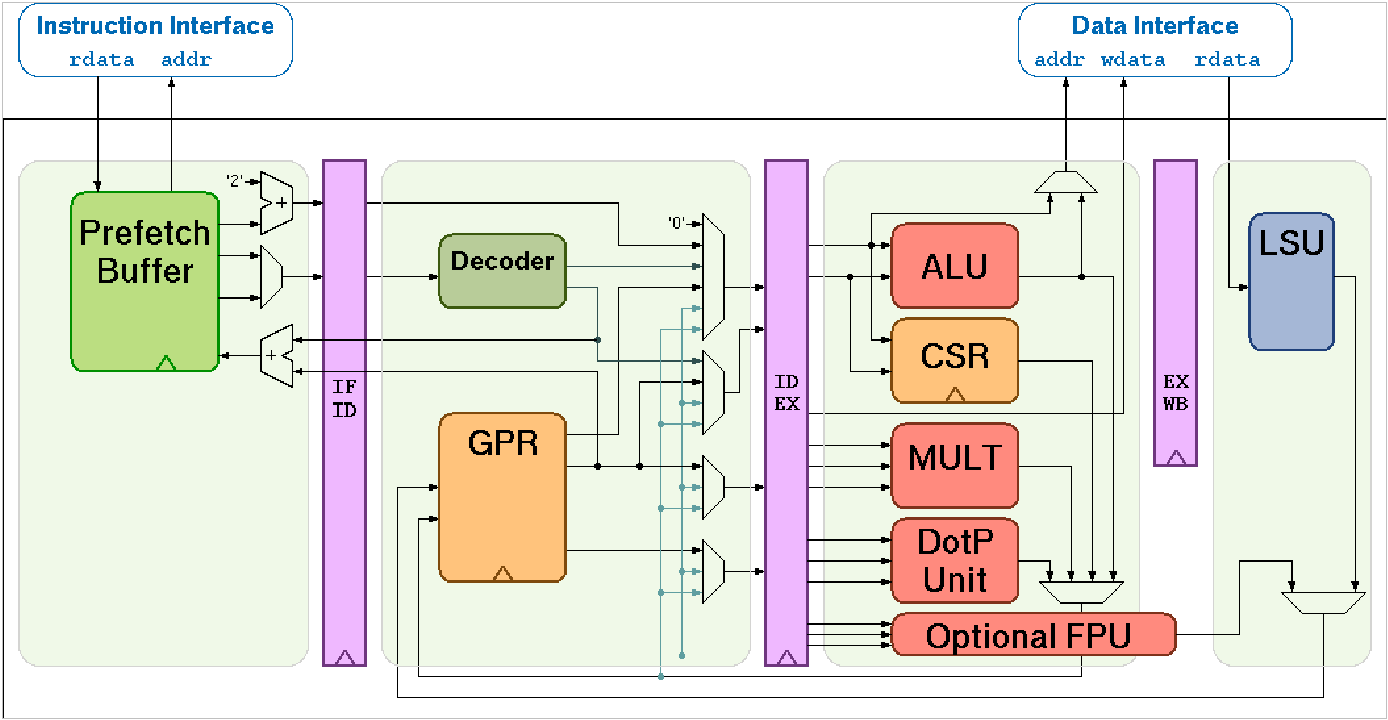
\includegraphics[width=\textwidth]{figures/pipeline.png}
    \caption{Schematics of RI5CY core}
    \label{fig:pipelined}
\end{figure}
\begin{figure}
    \centering
    % 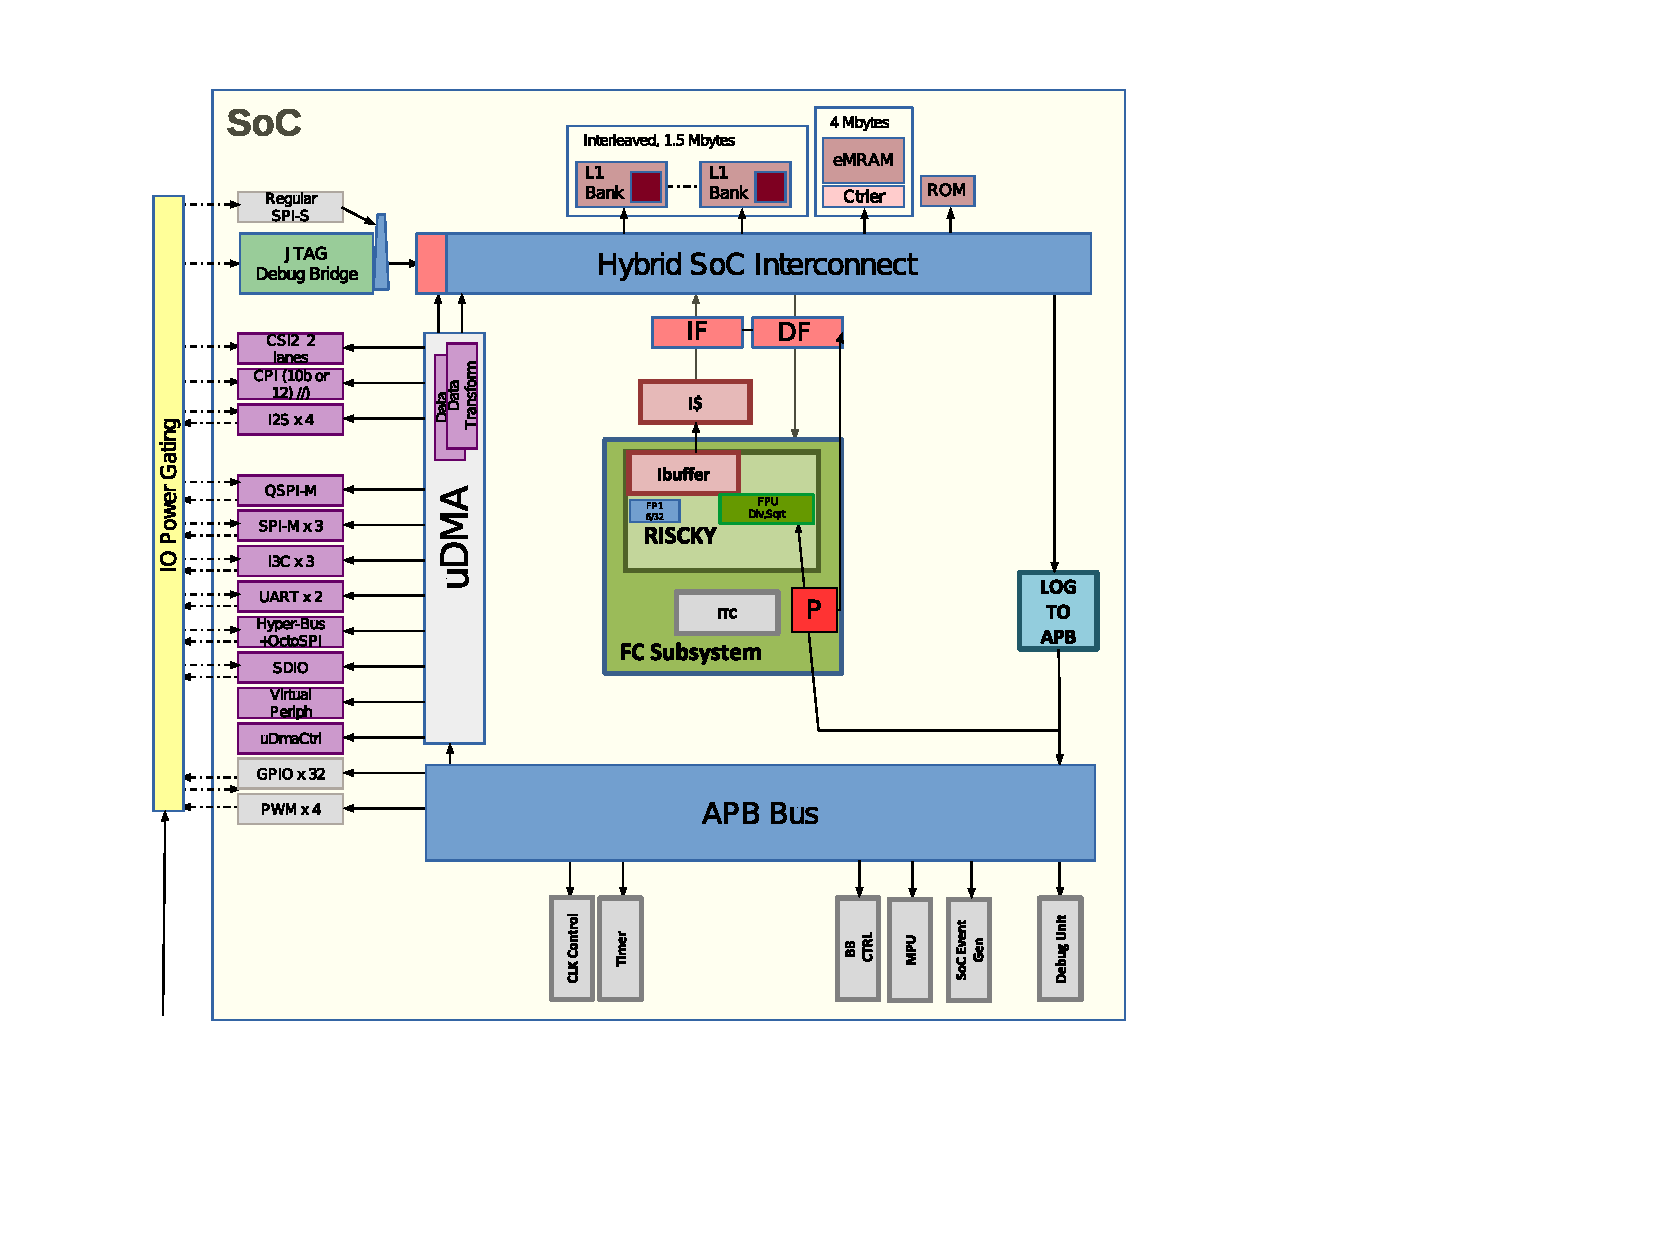
\includegraphics[trim={2.5cm 3.7cm 8.5cm 1.5cm},clip,width=\textwidth]{figures/top-level_vega_simplified.pdf}
    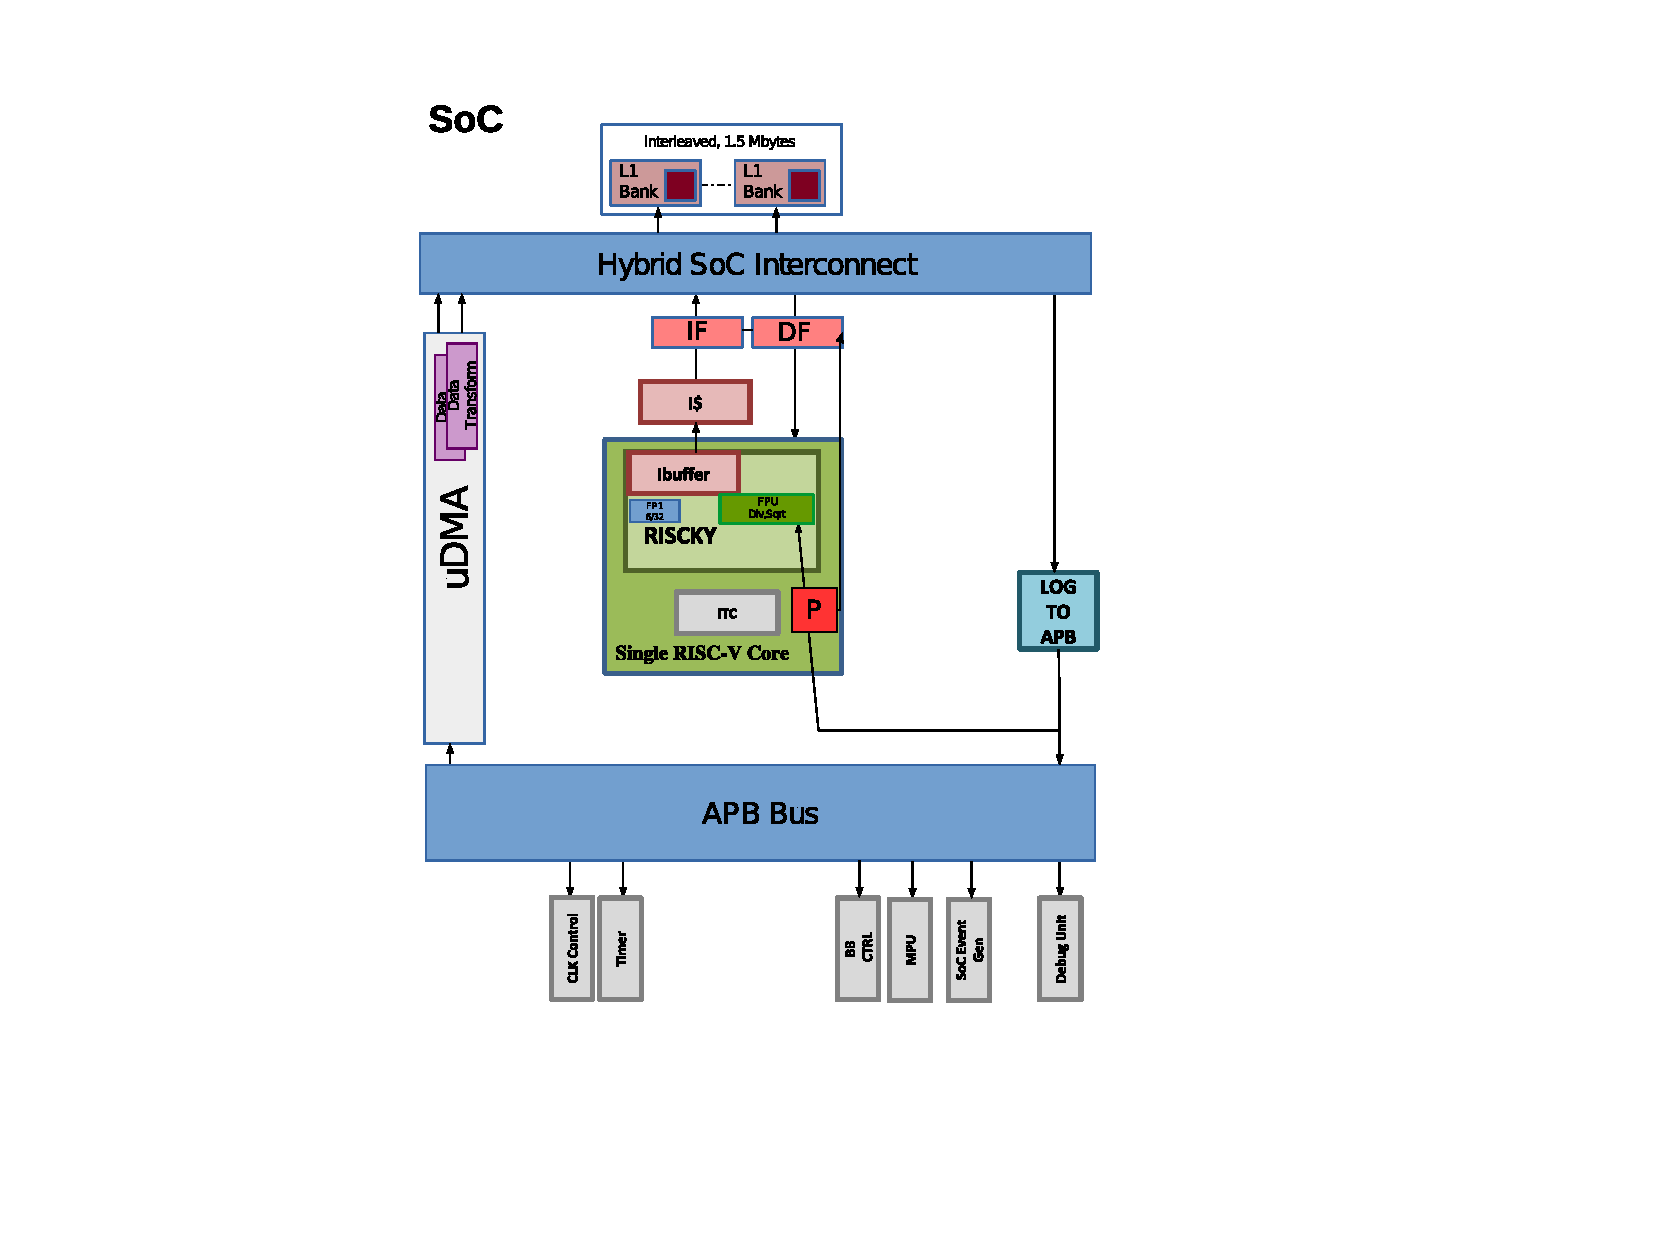
\includegraphics[trim={2.5cm 3.7cm 8.5cm 1.5cm},width=\textwidth]{figures/top-level_vega_simplified2.pdf}
    \caption{Top-Level RISC-V Architecture}
    \label{fig:top-level}
\end{figure}

% \begin{itemize}
%     \item 4-stage pipeline processor
%     \item RV32IMFCXpulp ISA
%     \item 70kGE + 30kGE FPU
%     \item Coremark/MHz 3.19
%     \item Floating Point Unit
%     \begin{itemize}
%         \item Iterative DIV/SQRT unit (7 cycles)
%         \item Pipeline MUL, ADD, SUB, Cast
%         \item Single cycle load, store, min, max, cmp etc.
%     \end{itemize}
% \end{itemize}
\section{PULP Toolflow}

PULP comes with an entire software toolflow. This includes PULP debug unit which allows to access the core with GDB or JTAG. On-chip performance counter are supported for a variety of metrics: Instructions counts, stalls (memory, branches, jump), statistics on branches (taken, not-taken) and number of memory accesses. Furthermore, the compiler infrastructure is based on the RISC-V GCC toolchain, extended to support custom instructions. Finally, the system can be fully simulated with the virtual platform which allows for very fast simulation and performance assessment compared to a RTL simulation and has a cycle-level divergence of less than 10\% and therefore enables fast prototyping.

% \todo{short introudction to the software toolflow}
% PULP Debug Unit via GDB/JTAG\\
% CSR, GPR, PC, performance counters (e.g. IPC, load stalls, …)\\
% GCC toolchain\\
% Our RISC-V compiler fully supports RI5CY custom ISA extensions\\
% Virtual Platform available for fast simulation and performance assessment (10\% wrt to cycle accurate)

\section{RI5CY Extensions}
The standard RISC-V ISA has been extended to speed up the very common execution patterns. The main extensions are described in the following:

Memory reads happen often in bursts which means that consecutive memory addresses have to be accessed. Often these addresses have to be calculated separately which introduces a high overhead of additional stalled cycles. To decrease this overhead RISC-V has been extended with a post increment load and post increment write. In this way the address pointer is incremented in hardware and no additional instructions are needed, which gives in average an overall speed up of 2x for memory accesses.

Also loops with few instructions inside have a high overhead, as the iteration variable has to be incremented and checked if the loop is finished. To reduce this overhead,  hardware loops have been introduced. Hardware loops are first configured with the number of iterations and the final instructions in a single cycle. This extension leads to just a 5\% area overhead while reaching an average speed up of 2x. Fig.\,\ref{fig:hwloops} shows a simple example where two nop instruction should be executed 100 times: with the special function lp.setupi the number of iterations are set to 100 and the PC pointer is set to the end of the loop.



\begin{figure}[h]
    \centering
    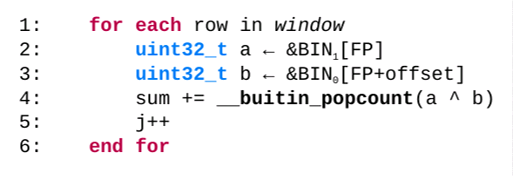
\includegraphics[width=.5\textwidth]{figures/builtin.png}
    \caption{Built-in functions allow to explicitly tell the compiler to place special-purpose instructions like popcount.}
    \label{fig:builtin}
\end{figure}

For some specific applications special bit manipulation instructions have been introduced. E.g. popcount returns the number of 1s in a integer register. These instructions are integrated into the software toolflow and intrinsic function (e.g. Fig.\,\ref{fig:builtin} shows an example for popcount) have been added.

For very low level optimization the asm directive (standard GCC function)  can be used to write assembly code within the C implementation.

Fixed-Point support have been added in the DSP extension (e.g. MAC with normalization and round).

The packet-SIMD extensions allows to pack several data into one 32-bit word. E.g. 2 16-bit words, 4 8-bit words or 8 4-bit words can be packed into a 32 bit register. Furthermore, a set of DSP extensions for pSIMD are supported like MIN, MAX, multiply-accumulate, multiply-subtract, dot product and others. Especially they can calculate ADD, SUB, MUL, MAC with fixed-point support including normalization and rounding. An example for a 16-bit word dot product is shown in Fig.\,\ref{fig:simd}, where as the upper 16 bits of both source registers are multiplied and then added to the product of the lower 16-bits.
% DSP extensions\\
% ABS, CLIP/Saturation, MIN, MAX, MAC, MSU\\
% Fixed-Point Support: ADD, SUB, MUL, MAC with normalization/round

\begin{figure}
    \centering
    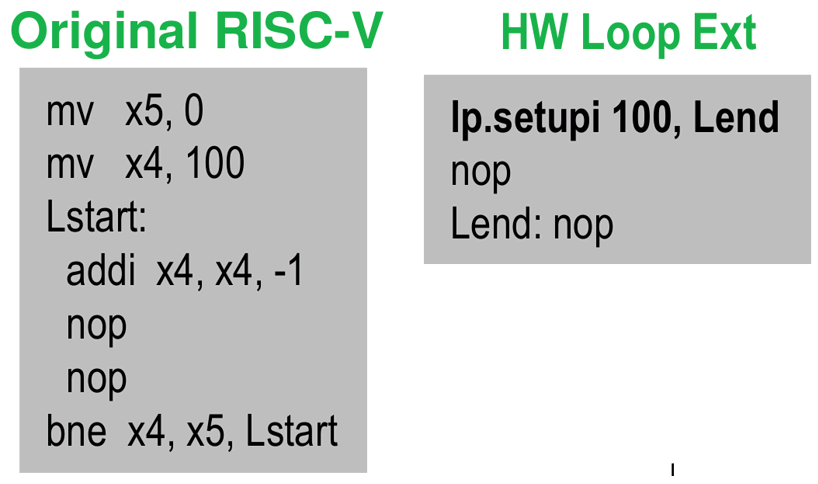
\includegraphics[width=.4\textwidth]{figures/hwloops.png}
    \caption{Hardware Loops: Example how number of instructions are reduced.}
    \label{fig:hwloops}
\end{figure}

% Packet-SIMD extensions\\
% 32-bit register is mapped to 4x8-bit words or 2x16-bit words\\
% Compute Instr. like add, sub, shift, avg, abs, dot product\\
% Compare Instr. like min, max compare\\
% Vector Manipulation: Extract, Pack, Shuffle
\begin{figure}
    \centering
    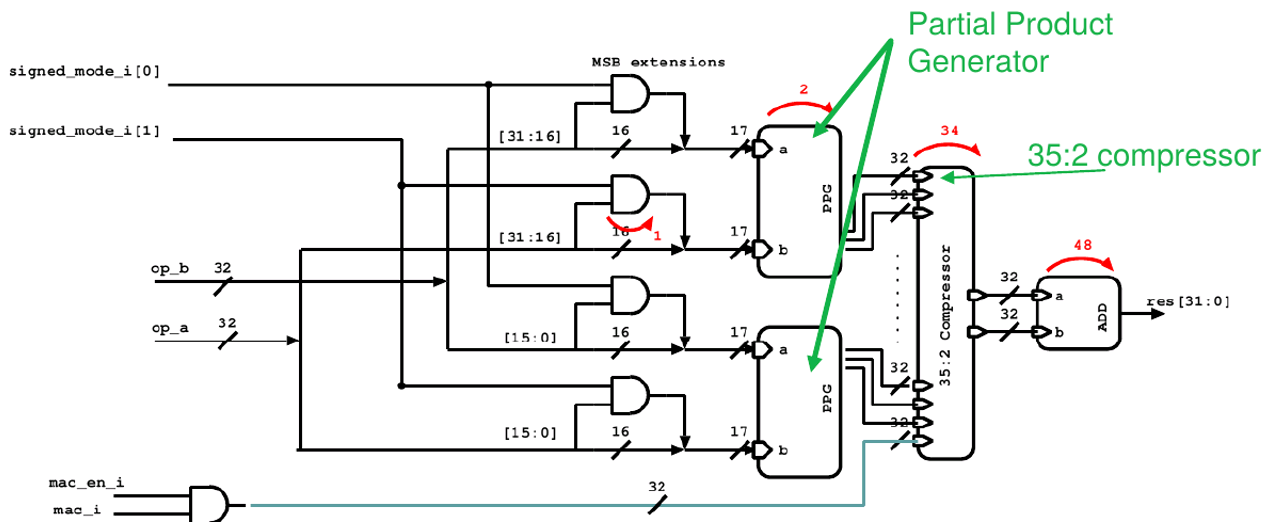
\includegraphics[width=\textwidth]{figures/simd.png}
    \caption{Dot-Product with packed SIMD. Upper half and lower half words are multiplied and summed together.}
    \label{fig:simd}
\end{figure}

% To allow for a straightforward integration of these extensions, there is 1) the custom RV32IMFCXpulp compiler and 2) software API extensions to use these extensions explicitly:

% There are explicit vector types for the SIMD extensions (e.g. 4 8-bit words can be packed into the data type v4qu), built-in functions (e.g. \_\_builtin\_popcount() ) or for low-level optimization the \texttt{asm} function (from the GCC standard).
% \todo{take pictures from slides. huawei\_kickOffLB.pptx}
\section{Implementation and Evaluation of the Benchmark Suite}
To allow for simple deployment of neural networks for sequential input data and general neural networks on RISC-V cores the project has been built in a modular way and split into the ML framework and RISC-V C implementation. 

There are plenty of Machine Learning platforms which have been developed by the community in recent years: TensorFlow, pyTorch, Caffe, etc. In this project, we use python as it is more open and extendable and used by the research community. PyTorch is also more flexible in deployment and debugging compared to its main competitor TensorFlow.

We have implemented the networks, as described on pyTorch and it serves as a golden model. We have implemented a toolflow to export these networks to RISC-V compilable C code including all the parameters in the right format (e.g. 16-bit fixed-point numbers or float).

On the RISC-V side, the basic kernels and neural network layers have been implemented and are discussed more in detail in the following section.
% \begin{itemize}
%     \item Machine Learning Framework (PyTorch)
%     \begin{itemize}
%         \item The networks have been implemented in pyTorch and can be calculated as a golden model.
%         \item The networks can be exported to RISC-V compilable C code.
%         \item The parameters and input FMs are stored in a C header file.
%         \item The network topology is stored in an array of a layer struct element which is also stored in the header file.
%     \end{itemize}
%     \item RISC-V implementations
%     \begin{itemize}
%         \item Commonly used functions (e.g. matrix-vector MAC) have been implemented.
%         \item Vector/Tensor functions (Vector add, Hadamard product, ...) have been implemented.
%         \item Linear Layer, RNN and LSTM have been implemented based on the basic operations.
%         \item A function which takes the networks and calculates all layers consecutively. 
%     \end{itemize}
    
   
% \end{itemize}


\subsection{Basic Building Blocks}
The code for the network layers (linear layer and LSTM) has been decomposed into smaller functions:
\begin{itemize}
\item \texttt{LinearLayer()}: calculates a matrix-vector multiplication (weights and input neurons) followed by a vector addition (bias).
\item \texttt{Two-LinearLayersAcc()}: To calculate the LSTM internal nodes ($f,i,o,g,h$) two linear layers are calculated and accumulated. To minimize writing back partial results to the L1 memory and read them again to accumulate with output of the second linear layer again, the Two-Linear basic block has been added. The output neurons are directly calculated, such that all the input neurons for the first and the second layer are weighted and accumulated, before next output neuron is calculated.
\item \texttt{HadMulTensor()}: calculates the point-wise multiplications of two Tensors which are needed to calculate the hidden nodes in LSTM and GRU cells.
\item \texttt{SigTensor()}: calculates the Sigmoid for every element of a Tensor.
\item \texttt{TanhTensor()}: Hyperbolic Tangent: calculates Hyperbolic Tangent for every element of a Tensor.
\end{itemize}

The layers are implemented as follows:
\begin{itemize}
    \item \texttt{LinearLayer()}: Calculates a fully connected layer (or MLP) which is identical to the basis function Linear.
    \item \texttt{RNNLayer()}: Calculates the RNN output based on the input feature map and set of weights and pointers (assigned by pointer). The hidden nodes are calculated and stored at the same address (in-place by pointer).
    \item \texttt{LSTMLayer()}: Calculates the LSTM layer, hidden nodes are calculated in-place (by pointer) and the internal nodes are calculated with the \texttt{Two-LinearLayersAcc()} function and hidden and cell nodes are calculated with the Hadamard product.
   \item \texttt{InferNetwork()}: Takes a list of layers which themselves include all relevant parameters (by pointer) and calculates the output of the network by layer-wise application of the right functions (\texttt{LSTMLayer()}, \texttt{LinearLayer()}, ...). Organizes pointers to input and output feature map in a ping-pong manner (pointer of the inputs neurons are set to the previous pointer of the output neurons).
\end{itemize}

\subsection{Results}
We have used the built-in performance counter and traces of the virtual platform to evaluate the performance. Tab.\,\ref{tab:numParam} shows the number of parameters, it can be seen that most of the networks have below 150\,k parameters, where as Ahmed et al. \cite{Ahmed2018} and Lee et al. \cite{Lee2018} have several million parameters, which will be needed to stored in off-chip memory. The benchmark suite requires 5.7\,MB memory to store all parameters for 16-bit words.

\begin{table}[h]
\centering
\begin{tabular}{|r|r|l|}
\hline

 [1] &        30k & \\ \hline
 [2] &         1k & \\ \hline
 [3] &       160k & \\ \hline
 [4] &        85k & \\ \hline
 [5] &         (0k) & entire topology unknown \\ \hline
 [6] &        24k & \\ \hline
 [7] &         1k & \\ \hline
 [8] &        37k & \\ \hline
[9] &      1'174k & // large network \\ \hline
[10] &    (4'032k) & CNN, external memory needed  \\ \hline
[11] &       150k & \\ \hline\hline
total &      1657k & \\ \hline
\end{tabular}
\caption{Number of Parameters}\label{tab:numParam}
\end{table}



% \begin{itemize}
%     % \item \todo{Note: instruction misses are currently not simuated by the virtual platform}
%     % \item IPC f 1.33
%     % \item the first two networks have LSTM introducing between 2.5-7.5\% of cycles
%     % \item most of stalls are based on waits for the memory
%     % \item 4.6 Mcycles for 3.5 Minstr.
%     % \item \todo{performance for 50 MHz ...}
%     % \item \todo{numParams}
% \end{itemize}
% analyze stalls (e.g. load, instruction misses)

To understand the number of active cycles and stalls, we have analyzed the stalls appearing while running the benchmark suite. Table\,\ref{tab:stalls} gives an overview. It can be seen that most of stalls are during memory accesses (24.6\% in average). The first two networks have small numbers of hidden nodes, which introduces a high overhead when a branch is taken and leads up to 7.5\% overhead in cycles for branches. The overall cycle per instruction (CPI) is 1.33.

\begin{table}[h]
\centering
\begin{tabular}{|r|r|r|r|r|r|r|r|r|}
\hline
          & MLP & LSTM & \#cycles & active & data stalls & branch stalls & others & CPI  \\ \hline
        %  & MLP & LSTM & total cycles & total instruction & data stall & oth stalls & CPI  \\ \hline
        %  & MLP & LSTM & total cycles & total instruction & data stall & branch stalls & oth stalls & CPI  \\ \hline
{[}1{]}  & 1   & 2    & 279.7 k      & 210.5 k           & 21.4\%      & 2.5\%          & 0.9\%       & 1.33 \\ \hline
{[}2{]}  & 2   & 1    & 11.4 k       & 8.7 k             & 13.1\%      & 7.2\%          & 3.0\%       & 1.30 \\ \hline
{[}3{]}  & 4   & 0    & 1282.3 k     & 963.9 k           & 24.8\%      & 0.0\%          & 0.0\%       & 1.33 \\ \hline
{[}4{]}  & 8   & 0    & 1361.3 k     & 1024.1 k          & 24.8\%      & 0.0\%          & 0.0\%       & 1.33 \\ \hline
{[}6{]}  & 6   & 0    & 188.1 k      & 141.9 k           & 24.5\%      & 0.0\%          & 0.0\%       & 1.33 \\ \hline
{[}7{]}  & 3   & 0    & 6.6 k        & 5.1 k             & 22.3\%      & 0.2\%          & 0.3\%       & 1.30 \\ \hline
{[}8{]}  & 4   & 0    & 291.6 k      & 219.6 k           & 24.7\%      & 0.0\%          & 0.0\%       & 1.33 \\ \hline
{[}11{]} & 4   & 0    & 1196.4 k     & 898.8 k           & 24.9\%      & 0.0\%          & 0.0\%       & 1.33 \\ \hline\hline
Total    & 32  & 3    & 4617.4 k     & 3472.7 k          & 24.6\%      & 0.2\%          & 0.1\%       & 1.33 \\ \hline
      \multicolumn{3}{|r|}{FPS@50MHz}       & 10.8 \ \ \       &  \multicolumn{5}{l}{}      \\ \cline{1-4}
\end{tabular}


\caption{Instruction and Cycle Count for the selected Benchmark Suite }\label{tab:stalls}
\end{table}



Tab.\,\ref{tab:funccalls} shows the number of cycles in the different basic function blocks. For the networks with no other than fully-connected layers, just the function \texttt{LinearLayer()} is executed and therefore not added in the table. For the networks containing LSTMs and RNNs, Tab.\,\ref{tab:funccalls} shows the function split with the amount of cycles in every instruction.
It can be seen that Sigmoid and Hyperbolic tangent take a lot of cycles within the LSTMs (e.g. 42\% in [2]) when calculated as Taylor expansion with 4 elements (row 1 and 3) and even with piece-wise linear approximation with 8 pieces (row 2 and 4) up to 33\%. Therefore, these functions seem are good candidates for further analysis on instruction acceleration. 

\begin{table}[h]
\begin{tabular}{|r|r|r|r|r|r|r|r|r|r|r|}
\hline
 \rotatebox{90}{network}    & \rotatebox{90}{\parbox{2cm}{approxim. model for\\ sig/tanh}}  & \rotatebox{90}{\#cycles} & \rotatebox{90}{MLP} & \rotatebox{90}{LSTM\ } & \rotatebox{90}{\texttt{LinearLayer()}\ }    & \rotatebox{90}{\texttt{LSTMLayer()}\ }    & \rotatebox{90}{\texttt{TwoLin...()}\ } & \rotatebox{90}{\texttt{SigTensor()}\ }    & \rotatebox{90}{\texttt{TanhTensor()}\ }   & \rotatebox{90}{Oth.\ } \\ \hline
{[}1{]} & taylor   & 279.7 k  & 1   & 2    & 14.4\% & 85.6\%  & 70.4\%    & 8.2\%  & 5.8\%  & 1.1\%  \\ \hline
{[}1{]} &  linear & 267.8 k      & 1   & 2    & 15.0\% & 85.0\%  & 73.5\%    & 6.2\%  & 4.1\%  & 1.2\%  \\ \hline

{[}2{]} & taylor   & 11.4 k   & 2   & 1    & 6.2\%  & 93.8\%  & 47.7\%    & 24.5\% & 17.4\% & 4.1\%  \\ \hline
{[}2{]} & linear  & 10.1 k       & 2   & 1    & 7.1\%  & 92.9\%   & 54.5\%    & 20.3\% & 13.3\% & 4.7\%  \\ \hline
\end{tabular}
\caption{Cycle statistic for basic blocks with sigmoid/hyperbolic tangent calculated either with taylor or piecewise linear approximation}\label{tab:funccalls}
\end{table}
% \begin{itemize}
%     \item Sigmoid and Tangens Hyperbolicus need a significant amount of cycles. up to 42\% of the entire calculation.
% \end{itemize}

Table \ref{tab:instr} shows the histogram of the instruction during execution of the benchmark suite with existing extensions. The code is calculating 480\,kMAC. There is just limited register re-use for data and weights and therefore for every MAC 2 data items have to be loaded, leading to  964\,k instructions for load (p.lh). The overhead for shifting back the multiplication results and additions for the fixed-point representation is quite high with a total of 960\,k instructions (30\%), which should be improved by using the intrinsic SIMD data types.

\begin{table}[h]
\centering
\begin{tabular}{|r|r|l|}
\hline
         Instr. & \# & Instruction description   \\ \hline
        p.lh& 964k & read 2 half words \\ \hline
       c.add& 494k & addition (16-bit compressed instr.) \\ \hline
         mul& 489k & 32bit to 32bit multiplication  \\ \hline
     p.exths& 480k & sign extension half-word \\ \hline
      c.srai& 480k & signed arithmetic right shift immediate \\ \hline
        c.mv&  22k & register to register copy \\ \hline
     other&  267k & other instructions \\ \hline\hline
         & 3'199k & total instructions \\ \hline
         & 4'294k & total \#cycles\\ \hline
\end{tabular}
\caption{Instruction and Cycle Count for the Benchmark Suite with extensions.}\label{tab:instr}
\end{table}
Table\,\ref{tab:instr_noopt} shows the instruction count if all the extension (SIMD and hardware loops and load/store increment) are turned off. It can be seen that 2.2x more cycles are needed, especially a lot of cycles are used to calculate addresses (i.e. addi is a common instruction used for this), furthermore the branch instruction appears on the top instruction as looping is common in the calculation of neural networks and this overhead is much lower in the version with the extensions turned on.

\begin{table}[h]
\centering
\begin{tabular}{|r|r|l|}
\hline
      c.addi& 1'425k & add immediate (mostly for address calculation) \\ \hline
          lh& 1'418k & (single)load half word \\ \hline
         bne& 713k & branch not equal \\ \hline
       c.add& 712k & addition\\ \hline
      c.slli& 708k & shift left immediate\\ \hline
      c.srai& 708k & signed arithmetic right shift immediate (16-bit compressed instruction) \\ \hline
         mul& 707k & 32bit to 32bit multiplication \\ \hline
        srai& 707k & signed arithmetic right shift immediate \\ \hline
        c.mv&  12k & register to register copy \\ \hline
others & 41k & other instructions \\ \hline\hline
         & 7'151k & total instructions \\ \hline
         & 9'283k & total \#cycles\\ \hline
\end{tabular}
\caption{Instruction and Cycle Count for the Benchmark Suite with no extensions}\label{tab:instr_noopt}
\end{table}




\subsection{Next Steps}
For the next steps in the project, we want to analyze more in details exact instruction patterns. E.g. instructions which follow each other very often and could be merged to a single instruction. Furthermore hyperbolic tangent and sigmoid take a high ratio of the instructions within LSTMs, GRU and RNN and the number of instruction can be reduced using piece-wise linear approximation, but we have to analyze the error we introduce by this approximation and how many pieces should be used.

Currently, the networks in [9] and [10] are not implemented because their parameters don't fit on-chip memory leading to external memory accesses. We will also implement these networks with a virtually larger memory (i.e. ideal memory reference) and with external memory accesses (e.g. hyperRAM) and DMA transfer.

There is still a high overhead in the fixed-point operations, with the existing SIMD data types these fixed-point shifting and sign-extension should be reduced. Then we will explore low-bit data types and floating-point operations before we will finally extend the ISA based on the instruction patterns found in the evaluation. These ISA extensions will be implemented in RTL. Furthermore, the assembler and compiler will be extended such that simple deployment from networks in C is enabled on the extended RISC-V core.

% \begin{table}[h]
% \begin{tabular}{|r|r|r|r|r|r|r|r|r|r|r|}
% \hline
%         & total cycles & MLP & LSTM & MLP    & LSTM   & Linear & TwoLinear & Sig    & Tanh   & Others \\ \hline
% {[}1{]} & 267.8 k      & 1   & 2    & 15.0\% & 85.0\% & 15.0\% & 73.5\%    & 6.2\%  & 4.1\%  & 1.2\%  \\ \hline
% {[}2{]} & 10.1 k       & 2   & 1    & 7.1\%  & 92.9\% & 7.2\%  & 54.5\%    & 20.3\% & 13.3\% & 4.7\%  \\ \hline
% \end{tabular}
% \caption{Linear Approximation of Sigmoid and Tanh }
% \end{table}
